\documentclass{article}

% Language setting
% Replace `english' with e.g. `spanish' to change the document language
\usepackage[spanish]{babel}

% Set page size and margins
% Replace `letterpaper' with `a4paper' for UK/EU standard size
\usepackage[letterpaper,top=2cm,bottom=2cm,left=3cm,right=3cm,marginparwidth=1.75cm]{geometry}

% Useful packages
\usepackage{amsmath}
\usepackage{graphicx}
\usepackage[colorlinks=true, allcolors=blue]{hyperref}
\usepackage{textgreek}
\usepackage{verbatim}
\usepackage{caption}
\usepackage{subcaption}
\usepackage{float}
\usepackage{array}

\begin{document}
\begin{titlepage}
\centering
{\bfseries\LARGE Universidad Politécnica de Valencia\par}
\vspace{1cm}
{\scshape\Large Escuela Técnica Superior de Ingeniería Informática\par}
\vspace{3cm}
{\scshape\Huge Lectura de llaves RFID-RC522 \par}
\vspace{3cm}
{\itshape\Large Proyecto Internet de las Cosas\par}
\vfill
{\Large Abel Haro Armero \par}
\vfill
{\Large Junio 2024 \par}
\date{}
\end{titlepage}



\tableofcontents


\section{Introducción}

Este proyecto consiste en desarrollar un sistema de control de acceso utilizando tecnología RFID (lector RFID-RC522).
El sistema permitirá registrar usuarios y controlar su acceso mediante llaves y tarjetas RFID. Para el cambio de modo del lector, entre registro o acceso, se utilizará comunicación Bluetooth. Los usuarios registrados y los accesos se mantendrán en una base de datos accesible mediante una API REST dentro de un contenedor. Para la visualización se utilizará Ubidots.

\begin{figure}[ht!]
\centering
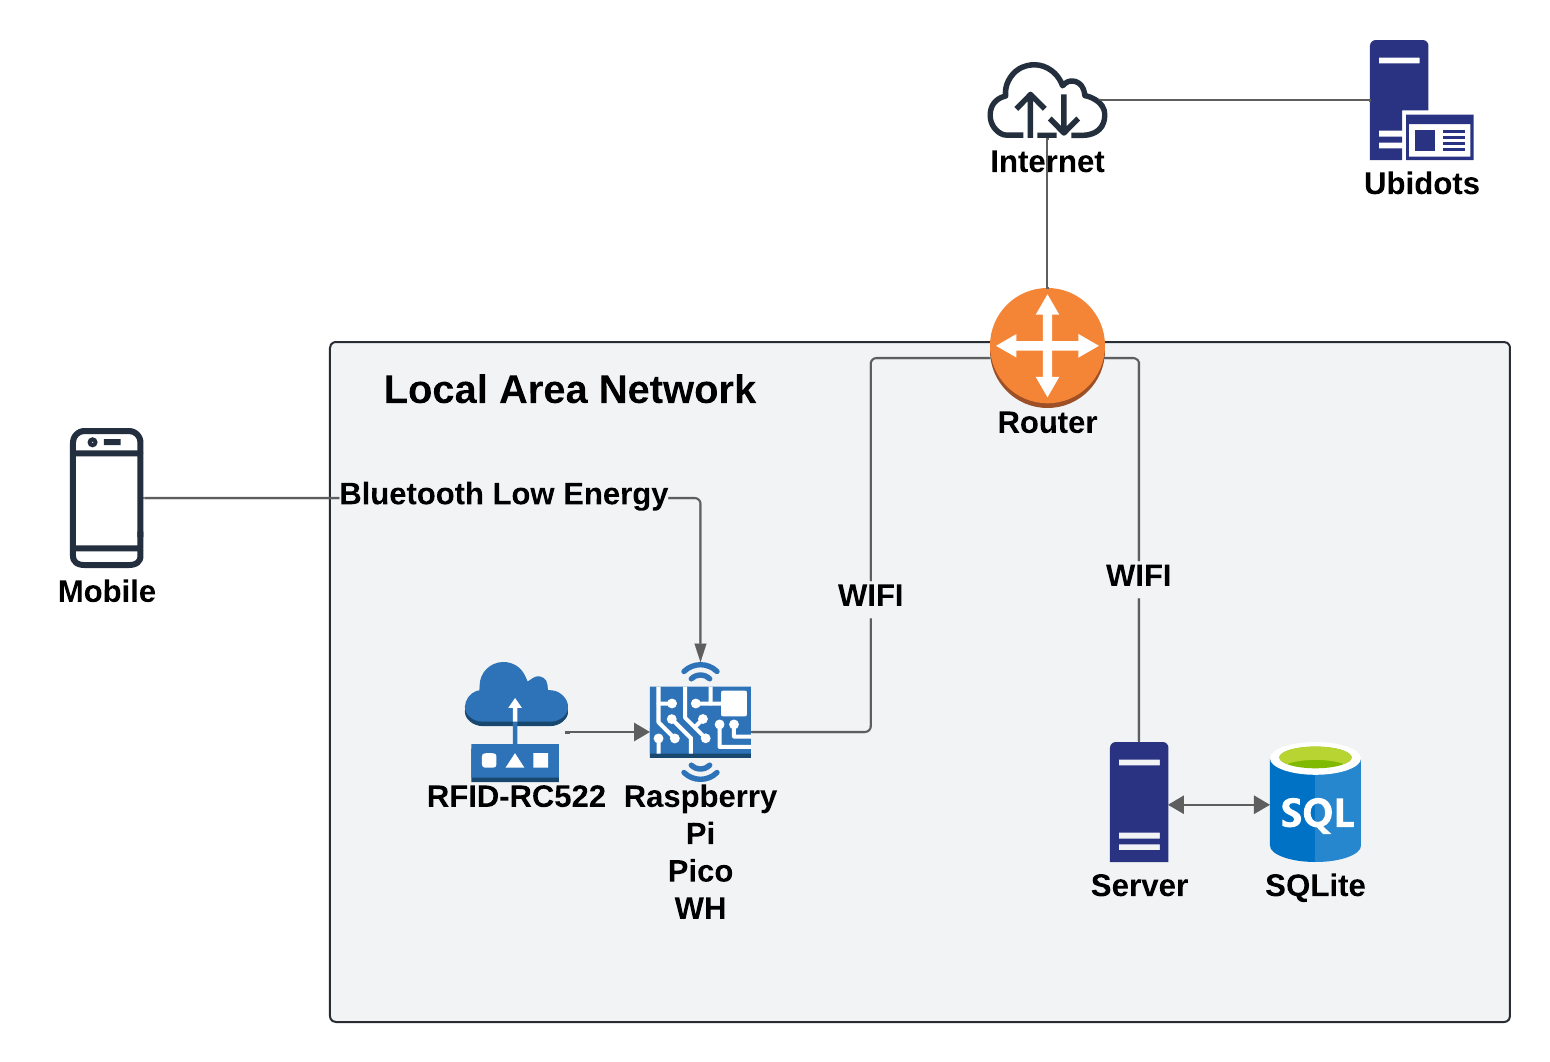
\includegraphics[width=0.9\linewidth]{../images/esquema_proyecto.png}
\caption{\label{fig:esquema red}Esquema del proyecto.}
\end{figure}

\section{Hardware utilizado}
Para el proyecto se ha utilizado el siguiente hardware:

\begin{figure}[!ht]
	\centering
	\begin{subfigure}[b]{0.45\textwidth}
		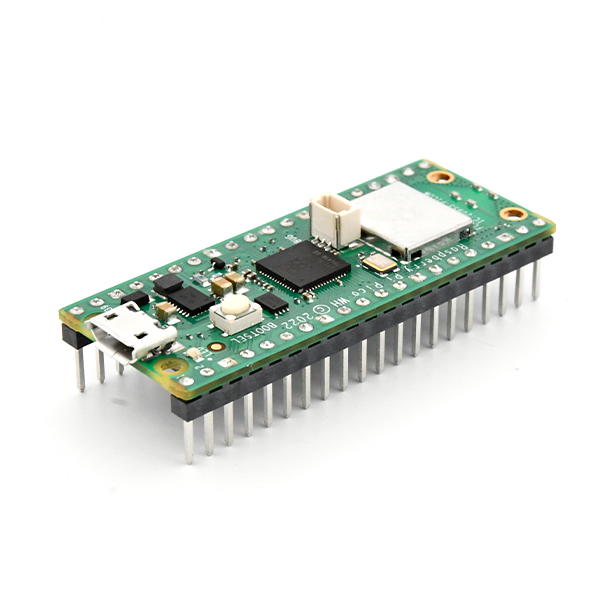
\includegraphics[width=\textwidth]{../images/picowh.png}
		\caption*{\href{https://www.raspberrypi.com/products/raspberry-pi-pico/}{Microcontrolador Raspberry Pi Pico WH}}
		\label{fig:picowh}
	\end{subfigure}
	\hfill
	\begin{subfigure}[b]{0.45\textwidth}
		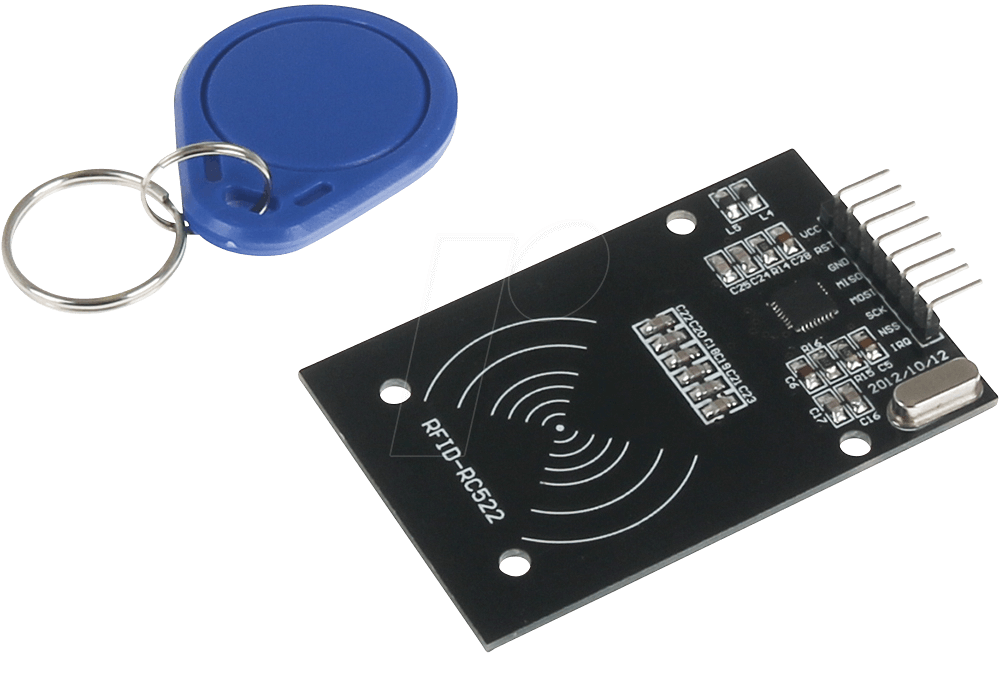
\includegraphics[width=\textwidth]{../images/mfrc522.png}
		\caption*{\href{https://www.keyestudio.com/products/keyestudio-mfrc522-rfid-s50-fudan-card-ic-card-module-with-spi-port-for-arduino-uno-r3-mega-2560-r3}{Lector de radiofrecuencia RFID-RC522}}
		\label{fig:MFRC522}
	\end{subfigure}
\end{figure}

\begin{figure}[!ht]
	\centering
	\begin{subfigure}[b]{0.45\textwidth}
		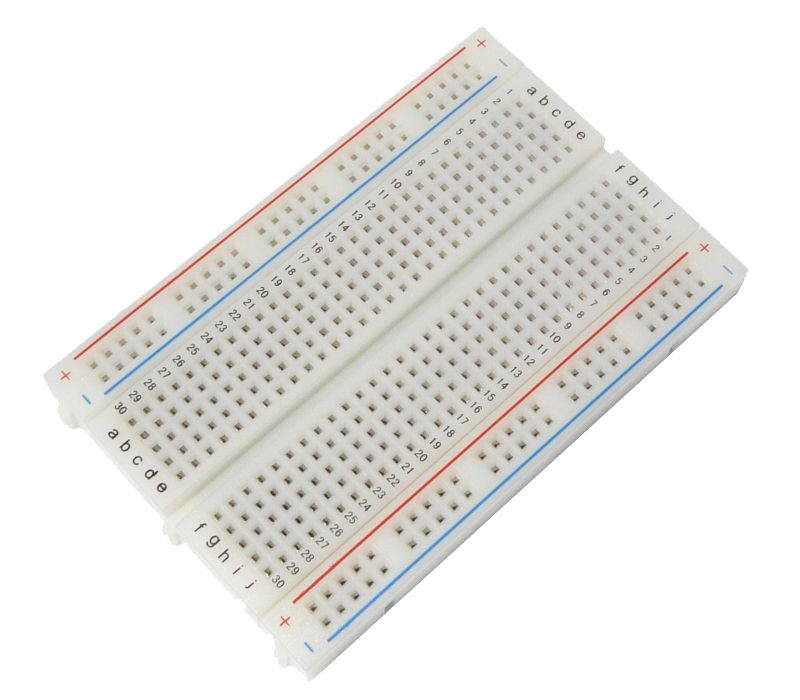
\includegraphics[width=\textwidth]{../images/protoboard.png}
		\caption*{Protoboard}
		\label{fig:protoboard}
	\end{subfigure}
	\hfill
	\begin{subfigure}[b]{0.45\textwidth}
		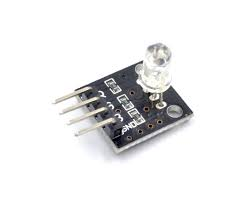
\includegraphics[width=\textwidth]{../images/led_tricolor.jpg}
		\caption*{Led tricolor KY-016 SP00}
		\label{fig:led tricolor}
	\end{subfigure}
\end{figure}

\begin{figure}[!ht]
	\centering
	\begin{subfigure}[b]{0.3\textwidth}
		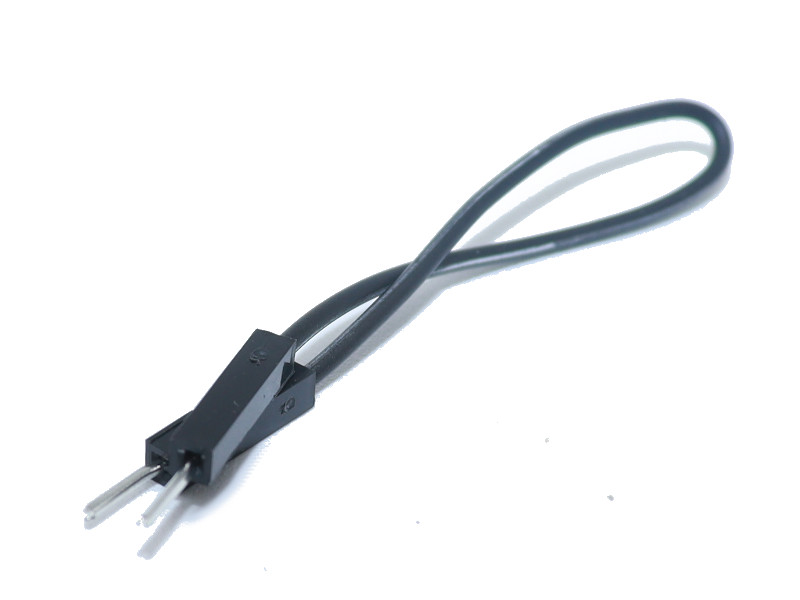
\includegraphics[width=\textwidth]{../images/cable_mm.jpg}
		\caption*{Cable Dupont Macho-Macho x3}
		\label{fig:cable mm}
	\end{subfigure}
	\hfill
	\begin{subfigure}[b]{0.3\textwidth}
		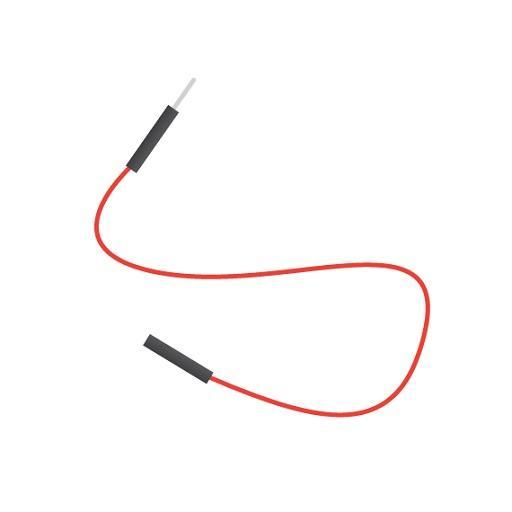
\includegraphics[width=\textwidth]{../images/cable_mh.jpg}
		\caption*{Cable Dupont Hembra-Macho x5}
		\label{fig:cable mh}
	\end{subfigure}
	\hfill
	\begin{subfigure}[b]{0.3\textwidth}
		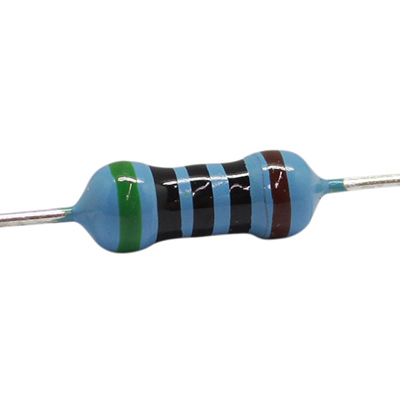
\includegraphics[width=\textwidth]{../images/resistencia.jpg}
		\caption*{Resistencia de 500\textOmega\ x2}
		\label{fig:resistencia}
	\end{subfigure}
\end{figure}


\section{Software utilizado}
\subsection{Microcontrolador}
Se empleó el microcontrolador Raspberry Pi Pico WH utilizando el lenguaje Micropython. Se hizo uso de las \href{https://github.com/micropython/micropython/tree/master/examples/bluetooth}{bibliotecas BLE} (Bluetooth Low Energy) para establecer y gestionar la comunicación Bluetooth en el microcontrolador. Para el dispositivo móvil se utilizó la aplicación \href{https://play.google.com/store/apps/details?id=de.kai_morich.serial_usb_terminal&pcampaignid=web_share}{Serial Bluetooth Terminal} disponible en Play Store. Para la lectura de llaves y tarjetas basadas en radiofrecuencia se utilizó la \href{https://github.com/danjperron/micropython-mfrc522/blob/master/mfrc522.py}{bibilioteca MFRC522}. En la comunicación con el servidor se implementó una API REST que permite el envío y recepción de datos de manera estructurada. Por último, se hizo uso de la librería machine para encender y apagar LEDs.

\subsection{Servidor}
En la implementación del servidor se hace uso de un contenedor Docker con la imagen base de Ubuntu. A la imagen se le instala Python junto con el paquete Flask para gestionar la lógica del servidor mediante solicitudes HTTP. Para la persistencia de datos se emplea un volumen de Docker junto con una base de datos SQLite.


\subsection{Ubidots}
Para la plataforma de se ha utilizado \href{https://stem.ubidots.com/}{Ubidots} mediante una cuenta STEM. Ubidots permite la visualización de datos en tiempo real y un envío de 1 req/s.

\section{Pasos para realizar el proyecto}
Para la realización del proyecto se deben seguir los siguientes pasos.
\subsection{Paso 1: Preintstalación de software necesario}
\textbf{Instalaciones de aplicaciones en el servidor:}
\begin{enumerate}
    \item Instalar \href{https://thonny.org/}{Thonny}.
    \item Instalar \href{https://code.visualstudio.com/download}{Visual Studio Code}.
    \item Instalar \href{https://docs.docker.com/get-docker/}{Docker}.
    \item Instalar \href{https://kinsta.com/es/base-de-conocimiento/instalar-python/}{intérprete de Python}.
\end{enumerate}


\textbf{Instalación de archivos en la Raspberry Pi Pico WH:}
\begin{enumerate}
	\item Instalar firmware de MicroPython:
		\begin{enumerate}
			\item Introducir el USB en el ordenador mientras se aprieta el botón BOOTSEL.
			\item Abrir Thonny y realizar los siguientes pasos:
			\begin{figure}[H]
			\centering
			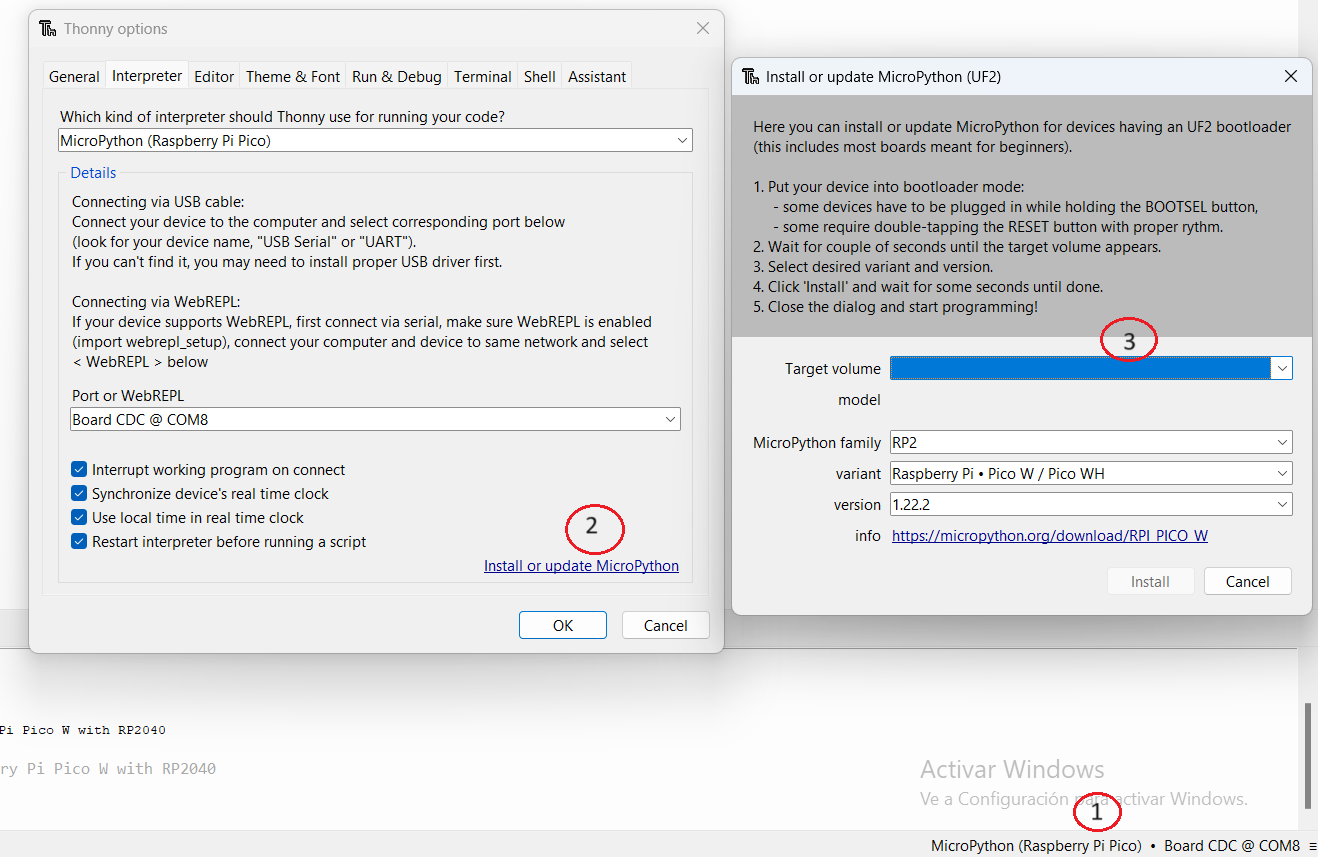
\includegraphics[width=0.8\linewidth]{../images/instalacion_firmware.png}
			\caption{\label{fig:instalación firmware}Pasos para la instalación del firmware.}
			\end{figure}
		\end{enumerate}
			\item Copiar el contenido de la carpeta \texttt{``microcontrolador''} del proyecto en la Raspberry Pi Pico WH.
\end{enumerate}

\textbf{Resgistro y configuración de Ubidots:}
\begin{enumerate}
	\item Crear una cuenta en \href{https://stem.ubidots.com/}{Ubidots Stem}.
	\item Crear un nuevo dispositivo.
	\begin{figure}[H]
		\centering
		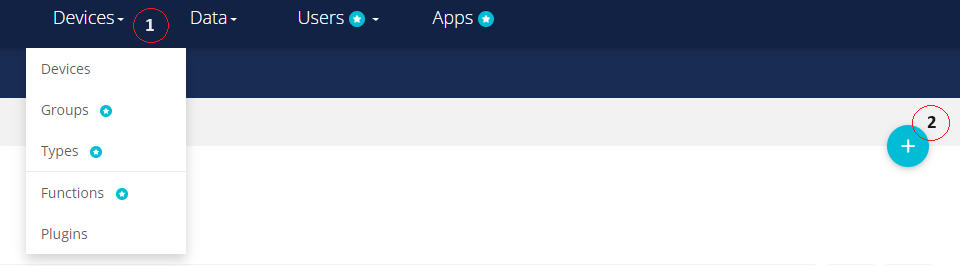
\includegraphics[width=0.7\linewidth]{../images/ubidots_create_device_1.png}
		\caption{\label{fig:ubidots_create_device_1}Creación de un nuevo dispositivo en Ubidots.}
	\end{figure}
	\item Añadir el nombre del dispositivo a la variable  \texttt{``DISPOSITIVE\_NAME''} dentro del archivo \texttt{``api/ubidots.py''}.
	\item Dentro del dispositivo crear dos raw variable, una para el registro de usuarios y otra para el registro de accesos de los usarios.
	\begin{figure}[H]
		\centering
		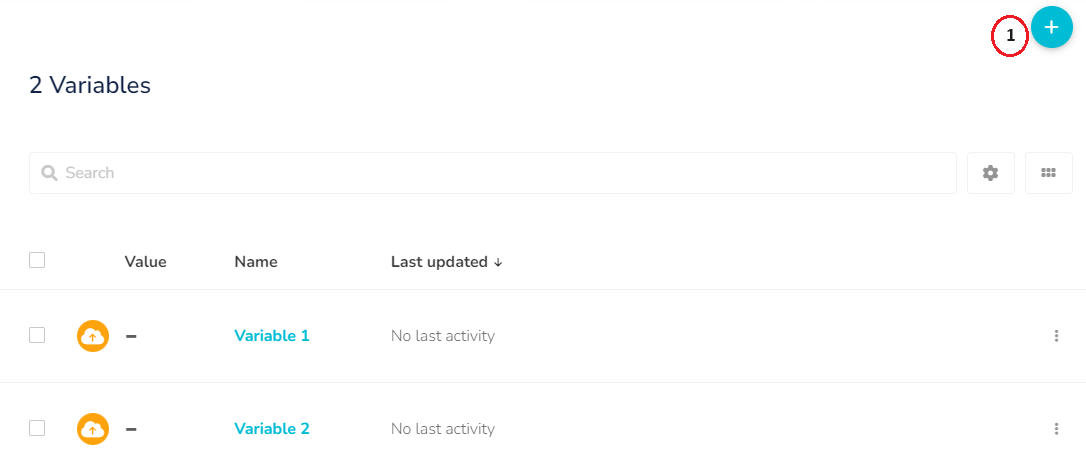
\includegraphics[width=0.7\linewidth]{../images/ubidots_create_variable.png}
		\caption{\label{fig:ubidots_create_variable_1}Creación de una variable en Ubidots.}
	\end{figure}
	\item Obteber el token de la API.
		\begin{figure}[H]
			\centering
			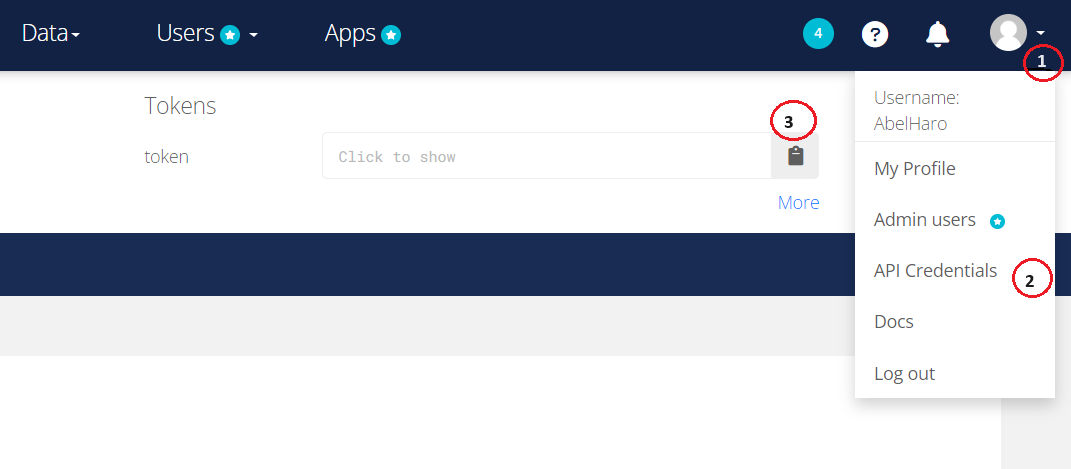
\includegraphics[width=0.7\linewidth]{../images/ubidots_obtener_token.png}
			\caption{\label{fig:ubidots_obtener_token}Obtención del token de la API en Ubidots.}
		\end{figure}
	\item Copiar el token de la API a la variable \texttt{``TOKEN\_UBIDOTS''} dentro del archivo \texttt{``api/ubidots.py''}.
\end{enumerate}

\subsection{Paso 2: Montaje circuito}
Conectar el lector RFID-RC522 a la Raspberry Pi Pico WH siguiendo la siguiente tabla:

\begin{center}
\begin{tabular}{|c|c|}
	\hline
	\textbf{Lector RFID-RC522} & \textbf{Raspberry Pi Pico WH} \\
	\hline
	VCC & 3.3V \\
	\hline
	RST & GP0 \\
	\hline
	GND & GND \\
	\hline
	IRQ & No conectado \\
	\hline
	MISO & GP4 \\
	\hline
	MOSI & GP3 \\
	\hline
	SCK & GP2 \\
	\hline
	SDA & GP1 \\
	\hline
\end{tabular}
\end{center}

Conectar el LED tricolor KY-016 SP00 a la Raspberry Pi Pico WH siguiendo la siguiente tabla:
\begin{center}
	\begin{tabular}{|c|c|}
		\hline
		\textbf{KY-016 SP00} & \textbf{Raspberry Pi Pico WH} \\
		\hline
		R & GP13 \\
		\hline
		G & GP12 \\
		\hline
		B & No conectado \\
		\hline
		- & GND \\
		\hline
	\end{tabular}
	\end{center}



El montaje del circuito debe quedar como se muestra en la siguiente figura:
\begin{figure}
	\centering
	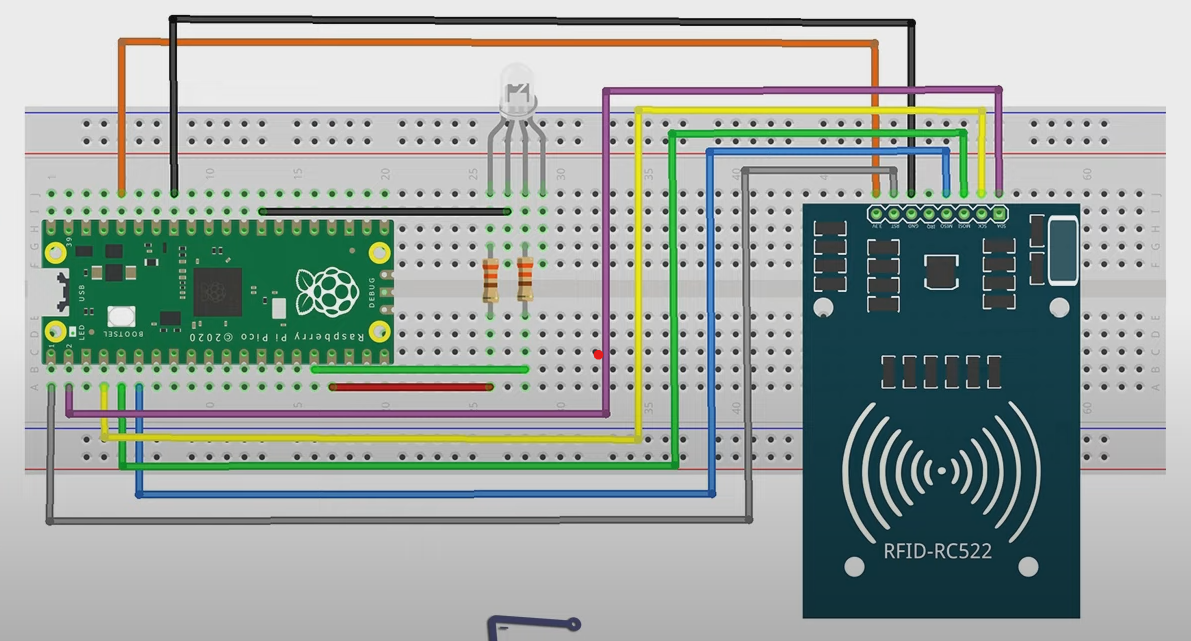
\includegraphics[width=1\linewidth]{../images/esquema_de_conexionado.png}
	\caption{\label{fig:circuito}Esquema de conexionado del proyecto.}
\end{figure}

\section{Problemas encontrados}
\subsection{Problema 1: Dirección estática del servidor} 
\subsection{Problema 2}
\subsection{Problema 3}
\section{Referencias}
\end{document}
